\documentclass[12pt,a4paper]{article}
\usepackage[UTF8]{ctex}
\usepackage{amsmath,amssymb}
\usepackage{xcolor}
\usepackage{hyperref}
\usepackage{geometry}
\usepackage{graphicx}
\geometry{margin=2.5cm}

\title{Deutsch-Jozsa Algorithm}
\author{QuoNic}
\date{}

\begin{document}
\maketitle

\begin{center}
\textbf{Algorithms} | Difficulty: Intermediate | Time: 10 min
\end{center}

\tableofcontents
\newpage

\section{Why do we need it?}

Deutsch-Jozsa algorithm was the first to prove quantum computational advantage.

\subsection{Classical Limitations}
\begin{itemize}
  \item Classical algorithm needs $2^{n-1}+1$ queries to determine function type
  \item For $n$ qubits, classical needs exponential queries
\end{itemize}

\subsection{Quantum Advantages}
\begin{itemize}
  \item Deutsch-Jozsa only needs 1 query
  \item Provides exponential speedup
  \item Paradigm for quantum algorithm design
\end{itemize}

\subsection{Real-world Applications}
\begin{itemize}
  \item Quantum algorithm teaching
  \item Quantum advantage verification
  \item Quantum computing theory
\end{itemize}

\section{Quick Start}

\begin{verbatim}
from quonic.algorithms import deutsch_jozsa

# Determine if function is constant or balanced
result = deutsch_jozsa("balanced", n_qubits=3)
print(f"Function type: {result.type}")
\end{verbatim}

\textbf{Expected Output}:
\begin{verbatim}
Function type: balanced
\end{verbatim}

\section{Theory Deep Dive}

\subsection{Circuit Diagram}

\begin{center}
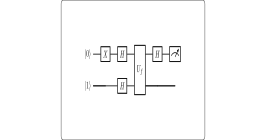
\includegraphics[width=0.6\textwidth]{../../images/deutsch_jozsa_circuit.svg}
\end{center}

\subsection{Mathematical Derivation}

Deutsch-Jozsa determines if function $f: \{0,1\}^n \to \{0,1\}$ is constant or balanced.

\textbf{Step 1: Initialization}
\begin{equation}
|\psi_0\rangle = |0\rangle^{\otimes n}|1\rangle
\end{equation}

\textbf{Step 2: Hadamard Gates}
\begin{equation}
|\psi_1\rangle = \frac{1}{\sqrt{2^n}} \sum_{x=0}^{2^n-1} |x\rangle \cdot \frac{|0\rangle - |1\rangle}{\sqrt{2}}
\end{equation}

\textbf{Step 3: Oracle Query}
\begin{equation}
|\psi_2\rangle = \frac{1}{\sqrt{2^n}} \sum_{x=0}^{2^n-1} (-1)^{f(x)} |x\rangle \cdot \frac{|0\rangle - |1\rangle}{\sqrt{2}}
\end{equation}

\textbf{Step 4: Hadamard and Measurement}

If measurement result is $|0\rangle^{\otimes n}$, function is constant; otherwise balanced.

\subsection{Geometric Interpretation}

Deutsch-Jozsa uses quantum superposition to query all inputs simultaneously, using interference to determine function type.

\section{Code Walkthrough}

\begin{verbatim}
from quonic.algorithms import deutsch_jozsa

# deutsch_jozsa(function_type, n_qubits)
# function_type: "constant" or "balanced"
# n_qubits: number of input qubits
result = deutsch_jozsa("balanced", n_qubits=3)

# result.type: "constant" or "balanced"
print(f"Function type: {result.type}")
\end{verbatim}

\section{Advanced Usage}

\subsection{Scenario 1: Constant Function}

\begin{verbatim}
from quonic.algorithms import deutsch_jozsa

# Constant function: f(x) = 0 for all x
result = deutsch_jozsa("constant", n_qubits=3)
print(f"Function type: {result.type}")
# Output: constant
\end{verbatim}

\subsection{Scenario 2: Balanced Function}

\begin{verbatim}
from quonic.algorithms import deutsch_jozsa

# Balanced function: f(x) = 0 for half x, 1 for other half
result = deutsch_jozsa("balanced", n_qubits=3)
print(f"Function type: {result.type}")
# Output: balanced
\end{verbatim}

\section{Use Cases}

\subsection{Quantum Algorithm Teaching}

Deutsch-Jozsa is a classic introductory quantum algorithm.

\subsection{Quantum Advantage Verification}

Deutsch-Jozsa was the first to prove quantum computational advantage.

\subsection{Quantum Computing Theory}

Deutsch-Jozsa is a paradigm for quantum algorithm design.

\section{FAQ}

\subsection{What is the speedup of Deutsch-Jozsa?}

Exponential speedup: classical needs $2^{n-1}+1$ queries, quantum only 1.

\subsection{What are the practical applications of Deutsch-Jozsa?}

Deutsch-Jozsa is mainly used for teaching and theoretical research, with limited practical applications.

\subsection{What are the limitations of Deutsch-Jozsa?}

Deutsch-Jozsa can only determine if function is constant or balanced, cannot handle other function types.

\section{Learning Path}

\subsection{Prerequisites}
\begin{itemize}
  \item Qubits and superposition
  \item Hadamard gate and CNOT gate
  \item Quantum measurement
\end{itemize}

\subsection{Next Steps}
\begin{itemize}
  \item Bernstein-Vazirani Algorithm
  \item Simon's Algorithm
  \item Shor's Algorithm
\end{itemize}

\section{Complete Examples}

\subsection{Example 1: Basic Deutsch-Jozsa}

\begin{verbatim}
from quonic.algorithms import deutsch_jozsa

result = deutsch_jozsa("balanced", n_qubits=3)
print(f"Function type: {result.type}")
\end{verbatim}

\section{Download}

\begin{itemize}
  \item [deutsch\_jozsa.py](https://github.com/ChrisLee0721/QuoNic/blob/main/examples/deutsch_jozsa/deutsch_jozsa.py)
\end{itemize}

\end{document}
